%Input preamble
%Style
\documentclass[12pt]{article}
\usepackage[top=1in, bottom=1in, left=1in, right=1in]{geometry}
\parindent 22pt
\usepackage{fancyhdr}

%Packages
\usepackage{adjustbox}
\usepackage{amsmath}
\usepackage{amsfonts}
\usepackage{amssymb}
\usepackage{bm}
\usepackage[table]{xcolor}
\usepackage{tabu}
\usepackage{color,soul}
\usepackage{makecell}
\usepackage{longtable}
\usepackage{multirow}
\usepackage[normalem]{ulem}
\usepackage{etoolbox}
\usepackage{graphicx}
\usepackage{tabularx}
\usepackage{ragged2e}
\usepackage{booktabs}
\usepackage{caption}
\usepackage{fixltx2e}
\usepackage[para, flushleft]{threeparttablex}
\usepackage[capposition=top,objectset=centering]{floatrow}
\usepackage{subcaption}
\usepackage{pdfpages}
\usepackage{pdflscape}
\usepackage{natbib}
\usepackage{bibunits}
\definecolor{maroon}{HTML}{990012}
\usepackage[colorlinks=true,linkcolor=maroon,citecolor=maroon,urlcolor=maroon,anchorcolor=maroon]{hyperref}
\usepackage{marvosym}
\usepackage{makeidx}
\usepackage{tikz}
\usetikzlibrary{shapes}
\usepackage{setspace}
\usepackage{enumerate}
\usepackage{rotating}
\usepackage{tocloft}
\usepackage{epstopdf}
\usepackage[titletoc]{appendix}
\usepackage{framed}
\usepackage{comment}
\usepackage{xr}
\usepackage{titlesec}
\usepackage{footnote}
\usepackage{longtable}
\newlength{\tablewidth}
\setlength{\tablewidth}{9.3in}
\setcounter{secnumdepth}{4}

\titleformat{\paragraph}
{\normalfont\normalsize\bfseries}{\theparagraph}{1em}{}
\titlespacing*{\paragraph}
{0pt}{3.25ex plus 1ex minus .2ex}{1.5ex plus .2ex}
\makeatletter
\pretocmd\start@align
{%
  \let\everycr\CT@everycr
  \CT@start
}{}{}
\apptocmd{\endalign}{\CT@end}{}{}
\makeatother
%Watermark
\usepackage[printwatermark]{xwatermark}
\usepackage{lipsum}
\definecolor{lightgray}{RGB}{220,220,220}
%\newwatermark[allpages,color=lightgray,angle=45,scale=3,xpos=0,ypos=0]{Preliminary Draft}

%Further subsection level
\usepackage{titlesec}
\setcounter{secnumdepth}{4}
\titleformat{\paragraph}
{\normalfont\normalsize\bfseries}{\theparagraph}{1em}{}
\titlespacing*{\paragraph}
{0pt}{3.25ex plus 1ex minus .2ex}{1.5ex plus .2ex}

\setcounter{secnumdepth}{5}
\titleformat{\subparagraph}
{\normalfont\normalsize\bfseries}{\thesubparagraph}{1em}{}
\titlespacing*{\subparagraph}
{0pt}{3.25ex plus 1ex minus .2ex}{1.5ex plus .2ex}

%Functions
\DeclareMathOperator{\cov}{Cov}
\DeclareMathOperator{\corr}{Corr}
\DeclareMathOperator{\var}{Var}
\DeclareMathOperator{\plim}{plim}
\DeclareMathOperator*{\argmin}{arg\,min}
\DeclareMathOperator*{\argmax}{arg\,max}

%Math Environments
\newtheorem{theorem}{Theorem}
\newtheorem{claim}{Claim}
\newtheorem{condition}{Condition}
\renewcommand\thecondition{C--\arabic{condition}}
\newtheorem{algorithm}{Algorithm}
\newtheorem{assumption}{Assumption}
\renewcommand\theassumption{A--\arabic{assumption}}
\newtheorem{remark}{Remark}
\renewcommand\theremark{R--\arabic{remark}}
\newtheorem{definition}[theorem]{Definition}
\newtheorem{hypothesis}[theorem]{Hypothesis}
\newtheorem{property}[theorem]{Property}
\newtheorem{example}[theorem]{Example}
\newtheorem{result}[theorem]{Result}
\newenvironment{proof}{\textbf{Proof:}}{$\bullet$}

%Commands
\newcommand\independent{\protect\mathpalette{\protect\independenT}{\perp}}
\def\independenT#1#2{\mathrel{\rlap{$#1#2$}\mkern2mu{#1#2}}}
\newcommand{\overbar}[1]{\mkern 1.5mu\overline{\mkern-1.5mu#1\mkern-1.5mu}\mkern 1.5mu}
\newcommand{\equald}{\ensuremath{\overset{d}{=}}}
\captionsetup[table]{skip=10pt}
%\makeindex

\setlength\parindent{20pt}
\setlength{\parskip}{0pt}

\newcolumntype{L}[1]{>{\raggedright\let\newline\\\arraybackslash\hspace{0pt}}m{#1}}
\newcolumntype{C}[1]{>{\centering\let\newline\\\arraybackslash\hspace{0pt}}m{#1}}
\newcolumntype{R}[1]{>{\raggedleft\let\newline\\\arraybackslash\hspace{0pt}}m{#1}}



%Logo
%\AddToShipoutPictureBG{%
%  \AtPageUpperLeft{\raisebox{-\height}{
\includegraphics[width=1.5cm]{uchicago.png}}}
%}

\newcolumntype{L}[1]{>{\raggedright\let\newline\\\arraybackslash\hspace{0pt}}m{#1}}
\newcolumntype{C}[1]{>{\centering\let\newline\\\arraybackslash\hspace{0pt}}m{#1}}
\newcolumntype{R}[1]{>{\raggedleft\let\newline\\\arraybackslash\hspace{0pt}}m{#1}}

\newcommand{\mr}{\multirow}
\newcommand{\mc}{\multicolumn}

%\newcommand{\comment}[1]{}

%Other parameters
\newcommand{\noutcomes}{95}
\newcommand{\noutcomesexpp}{357}
\newcommand{\noutcomesexpm}{343}
\newcommand{\noutcomesexpf}{355}
\newcommand{\treatsubsabc}{$75\%$}
\newcommand{\treatsubscarec}{$74\%$}
\newcommand{\treatsubscaref}{$63\%$}

%Counts
%Males
\newcommand{\positivem}{$78\%$}
\newcommand{\positivesm}{$29\%$}

%Females
\newcommand{\positivef}{$78\%$}
\newcommand{\positivesf}{$31\%$}

%Counts, control substitution
%Males
\newcommand{\positivecsnm}{$47\%$}
\newcommand{\positivescsnm}{$15\%$}

\newcommand{\positivecsam}{$79\%$}
\newcommand{\positivescsam}{$29\%$}

%Females
%% no alternative
\newcommand{\positivecsnf}{$84\%$}
\newcommand{\positivescsnf}{$55\%$}

%% alternative
\newcommand{\positivecsaf}{$79\%$}
\newcommand{\positivescsaf}{$33\%$}

%Pooled

%Effects
%Males

%Females
\newcommand{\empf}{$8$}
\newcommand{\yearsedf}{$1.7$}



%Pooled

%CBA
%IRR
%Males
\newcommand{\irrm}{$15\%$}
\newcommand{\irrsem}{$5\%$}

%Females
\newcommand{\irrf}{$9\%$}
\newcommand{\irrsef}{$7\%$}

%Pooled
\newcommand{\irrp}{$13\%$}
\newcommand{\irrsep}{$5\%$}

%BC
%Males
\newcommand{\bcm}{$11.24$}
\newcommand{\bcsem}{$4.60$}

%Females
\newcommand{\bcf}{$2.35$}
\newcommand{\bcsef}{$1.09$}

%Pooled
\newcommand{\bcp}{$5.63$}
\newcommand{\bcsep}{$2.15$}

%NPV streams
%Pooled
\newcommand{\parincomenpvp}{$\$119,346$}

\newcommand*\leftright[2]{%
  \leavevmode
  \rlap{#1}%
  \hspace{0.5\linewidth}%
  #2}

\newcommand{\orth}{\ensuremath{\perp\!\!\!\perp}}%
\newcommand{\indep}{\orth}%
\newcommand{\notorth}{\ensuremath{\perp\!\!\!\!\!\!\diagup\!\!\!\!\!\!\perp}}%
\newcommand{\notindep}{\notorth}

\externaldocument{abc_comprehensivecba_appendix}
\pagenumbering{Roman}

\begin{document}
\doublespacing
\noindent \textbf{Section 6 Proposal}\\

\noindent \textbf{[JLG: Professor, I'm proposing major changes to Section 6. The version in which we left when you went to China was imprecise, in my opinion. It read too much as a cookbook and it didn't provide the reader with enough context for the proof of the Theorem to be straightforward, as we claim. With the changes I made, it is possible to derive the implications of each assumption after enunciating it and then the Theorem does follow. I'm providing a proof based on deriving these implications. I look froward to your comments. Given that the changes are major, I want to first propose them via this stand alone document.]}

\setcounter{section}{5}
\section{Predicting and Monetizing Life-cycle Costs and Benefits} \label{section:cbamethodology}

\noindent A central focus of this paper is on summarizing the multiple benefits of ABC/CARE using benefit/cost and rate of return analyses. This requires predicting the out-of-sample costs and benefits of the program over the life cycle after the measurement phase of the study ends. This is a fundamental problem in empirical social science that has been addressed in the literature in multiple ways.\footnote{See, e.g., \cite{Heckman_Lochner_ea_2006_HEE}. \citet{Heckman_Moon_etal_2010_RateofReturn} use a variety of methods to predict future labor income in the Perry Preschool Project. The various methods are in general agreement. They fit a variety of panel data labor income dynamics models and project future labor income with them.} This section explains our strategy for using multiple data sources to predict out-of-sample life-cycle costs and benefits of education, labor income, transfer income, crime, and health. Our approach build on and extends the analysis of \citet{Heckman_Pinto_etal_2013_PerryFactor}, who show that, in a similar setting to ours, the effect of treatment on outcomes operates through its effects on inputs in a stable production function rather than through shifts in the production function. We report and extend a similar finding for ABC/CARE.\\

\noindent To construct cost-benefit estimates we (i) \textit{interpolate} components not observed due to intermittent data collection; and (ii) \textit{extrapolate} (predict) components not observed because the follow-ups stop when the subjects were in their mid-30s. We use multiple sources of non-experimental data representative on the national or state level to construct these interpolations and extrapolations. Table~\ref{table:sources} presents the components for which we conduct these exercises and the data sources we use. We use labor income as running example for illustration purposes, but our methodology is the same for predicting the rest of the outcomes unless otherwise noted.

\begin{table}[!htbp]
\begin{threeparttable}
\caption{Auxiliary (Non-experimental) Data Sources for Interpolation and Extrapolation of Life-cycle Benefits and Costs} \label{table:sources}
\footnotesize
%\input{../../AuxilliaryFiles/Preamble}
%\newgeometry{margin=.1in}

%\newcolumntype{L}[1]{>{\raggedright\let\newline\\\arraybackslash\hspace{0pt}}m{#1}}
%\newcolumntype{C}[1]{>{\centering\let\newline\\\arraybackslash\hspace{0pt}}m{#1}}
%\newcolumntype{R}[1]{>{\raggedleft\let\newline\\\arraybackslash\hspace{0pt}}m{#1}}

\begin{tabular}{L{3cm} C{1cm} C{1cm} C{1cm} C{1cm} C{1cm} C{2cm}} \toprule
 & \multicolumn{6}{c}{Subject's Age} \\
\textbf{Component}  & 16--21 & 21--30 & 31--34 & 34--50 & 61--67 & 68--Death \\ \midrule
\textbf{Transfer Income} & & \multicolumn{1}{c}{\cellcolor[gray]{.8} cNLSY} & \multicolumn{3}{c}{\cellcolor[gray]{.7} NLSY79; PSID}  &  \\ \midrule
\textbf{Subject Income} & &  \multicolumn{1}{c}{\cellcolor[gray]{.8} cNLSY} & \multicolumn{3}{c}{\cellcolor[gray]{.7} NLSY79; PSID} & \\ \midrule
\textbf{Health}  & \multicolumn{6}{c}{\cellcolor[gray]{.8} PSID; MEPS; MCBS; HRS}     \\ \midrule
\textbf{Crime} & \multicolumn{4}{c}{\cellcolor[gray]{.8} NCDPS; NJRP; NVS; UCRS} \\ \bottomrule
\end{tabular}
%\end{document}
\begin{tablenotes}
\footnotesize
Note: This table details the non-experimental data sources we use to interpolate and extrapolate the life-cycle benefits and costs of ABC/CARE. CNLSY: Children of the National Longitudinal Survey of the Youth 1979; NLSY79: National Longitudinal Survey of the Youth 1979; PSID: Panel Study of Income Dynamics; MEPS: Medical Expenditure Panel Survey; MCBS: Medicare Current Beneficiary Survey; HRS: Health and Retirement Study; NCDPS: North Carolina Department of Public Safety Data; NVS: National Crime Victimization Survey; NJRP: National Judicial Reporting Program; UCRS: Uniform Crime Reporting Statistics.
\end{tablenotes}
\end{threeparttable}
\end{table}


\subsection{Using Auxiliary Data Sources to Predict Outcomes Out of Sample}\label{sec:usingaux}

\noindent This subsection provides an informal summary of our prediction procedure, and some informative tests. The rest of Section~\ref{section:cbamethodology} provides a formal theory for the prediction, as well as tests and several details. We recommend to the readers who are not interested in the formalization or the details to finish reading this subsection and skip to Section 7, in which we discuss results.\\

\noindent We have data on control- and treatment-group individuals through age $t^{\ast}$. We lack information on participant outcomes afterward. Yet, post-$t^{\ast}$ outcomes are required to construct counterfactual life-cycle profiles. We predict this outcomes based on three steps, roughly: (i) find counterparts to the treatment- and control-group individuals in the non-experimental sample to find synthetic control and treatment groups; (ii) fit the dynamic relationship between the vector of outcomes at time $t$ ($\bm{Y}^{d}_{i,t}$) and variables that could have been affected by treatment ($\bm{X}^{d}_{i,t}$), as well as background variables ($\bm{B}$); and (iii) use the dynamic relationship estimated in the non-experimental synthetic control and treatment groups to predict out-of-sample the post-$t^{\ast}$ outcomes.\\ 

\noindent To illustrate our procedure, Figure~\ref{fig:labor-income-profiles} displays the labor income life-cycle profiles \textit{predicted} for the treatment and control groups.\footnote{We use labor income as an illustration in this section because the life-cycle patterns are well-known in the literature and straightforward to compare between the experimental and non-experimental samples. We predict transfer income using this same procedure. See Section~7 for results.} It also displays the \textit{realized} and \textit{predicted} labor income at $t^*$. The agreement through $t^*$ is close. Our pattern of life-cycle labor incomes is typical for low-skilled workers \citep{Blundell-etal_2015_J-Pub-E,Gladden_Taber_2000_WageProgression,Sanders-Taber_2012_AR,Lagakos_Moll_etal_2016_LifeCycle_NBER}.\footnote{The prediction of labor (transfer) income is based on indicator variables of being male and being black, mother's education, average PIAT scores from ages 5 to 7, years of education at age 30, body-mass index at 34, labor (transfer) income at ages 21 and 30, and one-period lagged labor (transfer) income. As we explain in the next section, our prediction is based on a first-order Markov process. We use labor (transfer) income at age 21 to initialize this process. The age-30 observation helps us validate our procedure. A justification for the use of these variables, evidence on their predictive power, and a sensitivity analysis to using different prediction variables are in Appendix~\ref{appendix:methodology}. In this appendix and in Section 6.3, we also explain details on different predictions for parental income.}\\

\begin{sidewaysfigure}[!htbp]
\centering
\caption{Labor Income Profile Predictions}\label{fig:labor-income-profiles}
\begin{subfigure}[h]{0.5\textwidth}
		\centering
		\caption{Prediction for ABC/CARE Males} \label{fig:labor-income-profilesc}
		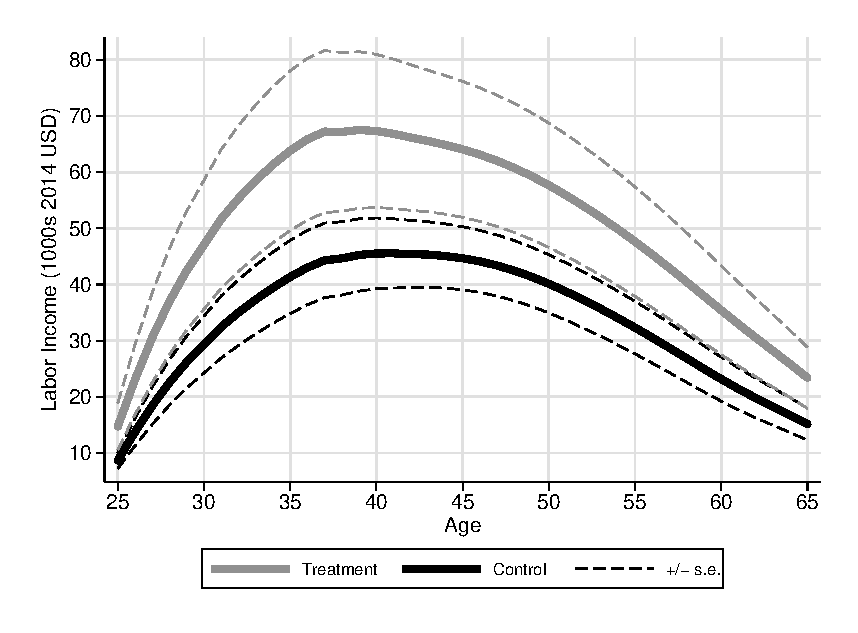
\includegraphics[width=\textwidth]{output/labor_25-65_pset1_mset3_male.eps}
\end{subfigure}%
\begin{subfigure}[h]{0.5\textwidth}
		\centering
		\caption{Prediction for ABC/CARE Females} \label{fig:labor-income-profilesa}
		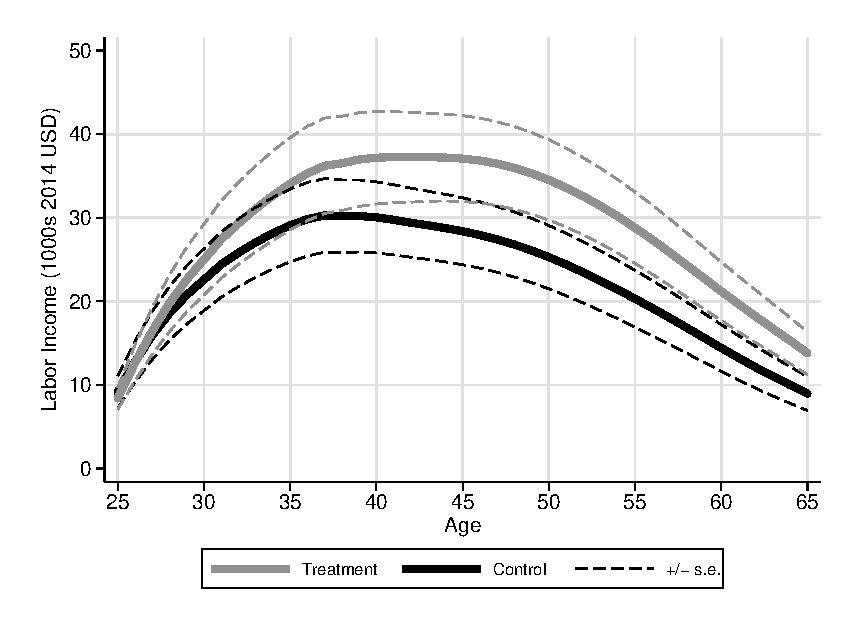
\includegraphics[width=\textwidth]{output/labor_25-65_pset1_mset3_female.eps}
\end{subfigure}
\footnotesize \justify
Note: Panels (a) displays the predicted labor income life-cycle profiles for ABC/CARE for males by treatment status, based on the method proposed in this section. We combine data from the Panel Study of Income Dynamics (PSID), the National Longitudinal Survey of Youth 1979 (NLSY79), and the Children of the National Longitudinal Survey of Youth 1979 (CNLSY79). We highlight the \textit{realized or observed} labor income at $t^*$ (age 30) for the ABC/CARE control- and treatment-group participants. Panel (b) displays the analogous figure for females. Standard errors are based on the empirical bootstrap distribution.  See Appendix~\ref{appendix:methodology} for a discussion of our choice of predictors and a sensitivity analysis to this choice.
\end{sidewaysfigure}

\noindent In the experimental sample, all of the parents of children with observed characteristics $\bm{B} \in \mathcal{B}_0$ agree to participate in the program. Since in the non-experimental sample there are no treatment group members, a test of the validity of our prediction procedure is to compare the labor incomes of individuals in the non-experimental sample for whom $\bm{B} \in \mathcal{B}_0$ to the labor incomes of the synthetic control group members (i.e., the groups in the non-experimental samples that we use to extrapolate control group outcomes). We also compare labor income at $t^*$ of both groups to the observed labor income in the experimental control group (we observe labor income at $t^*$). Figure~\ref{figure:controltests} makes these comparisons. We plot the labor income of individuals in our non-experimental sample such that $\bm{B} \in \mathcal{B}_0$ and the synthetic control group from ages 20 to 45. We also display the labor income of the experimental control group at $t^*$ (age 30).\footnote{The graphs stop at age 45 because we do not observe all of the components of the High Risk Index after age 45 in the non-experimental samples. We use only a subset of this index to make life-cycle projections. The subset variables are effective predictors over the range where the full set of $\bm{B}$ is available.}

\begin{sidewaysfigure}[!htbp]
\centering
\caption{Labor Income Profile, Disadvantaged Individuals Synthetic Control Group in the Non-experimental Samples}\label{figure:controltests}
\begin{subfigure}[h]{0.5\textwidth}
		\centering
		\caption{Males}
		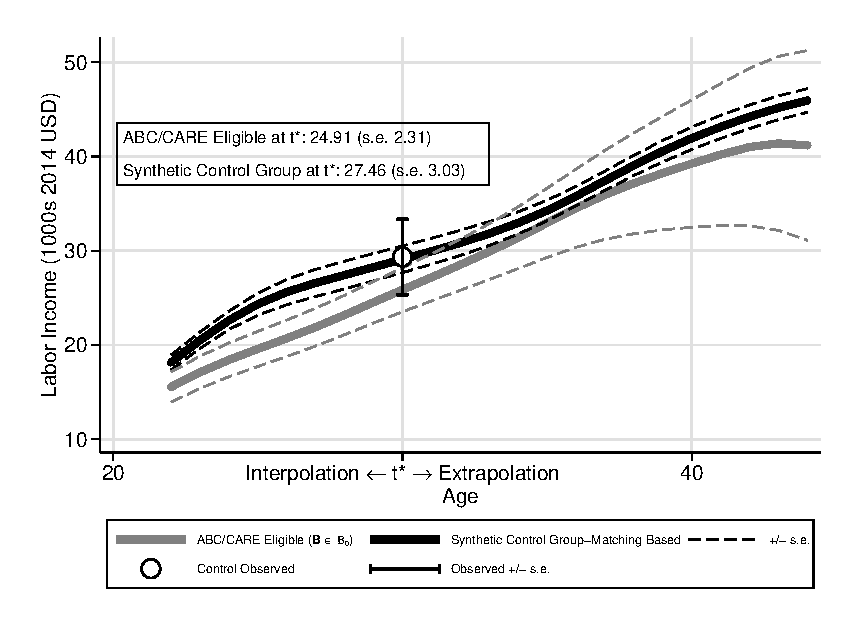
\includegraphics[width=\textwidth]{output/abccare_disad_1.eps}
\end{subfigure}%
\begin{subfigure}[h]{0.5\textwidth}
		\centering
		\caption{Females}
		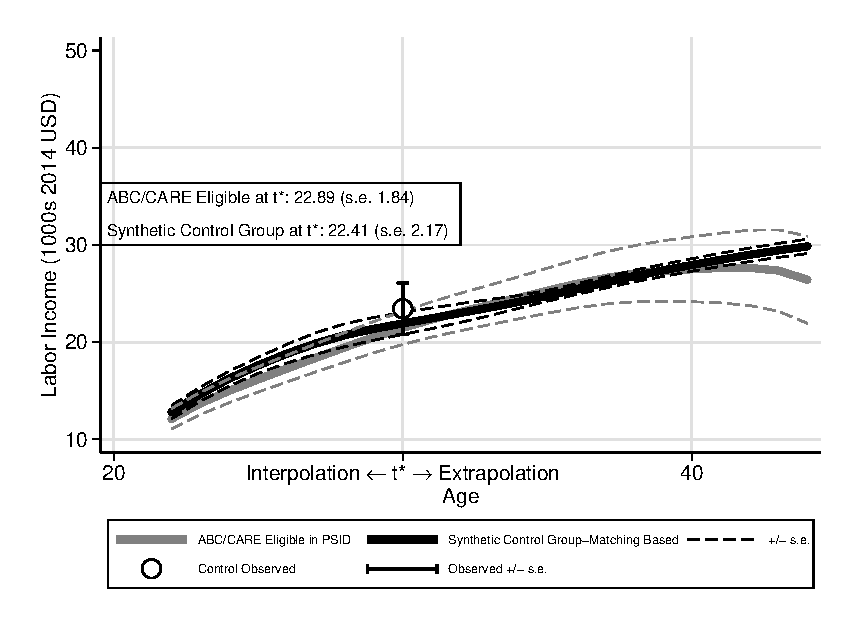
\includegraphics[width=\textwidth]{output/abccare_disad_0.eps}
\end{subfigure}
\footnotesize \justify
Note: Panels (a) displays the predicted labor income for males in the non-experimental samples such that $\bm{B} \in \mathcal{B}_0$, i.e. ABC/CARE eligible, and for the synthetic control group we construct based on the method proposed in this section. We combine data from the Panel Study of Income Dynamics (PSID), the National Longitudinal Survey of Youth 1979 (NLSY79), and the Children of the National Longitudinal Survey of Youth 1979 (CNLSY79). We highlight the \textit{realized or observed} labor income at $t^*$ (age 30) for the ABC/CARE control- and treatment-group participants. We stop at age 45 for want of data to compute the high-risk index defining $\bm{B} \in \mathcal{B}_0$ in ABC/CARE in the non-experimental samples. Panel (b) displays the analogous figure for females. Standard errors are based on the empirical bootstrap distribution.
\end{sidewaysfigure}

\subsection{Justifying the Matching Procedure} \label{section:just}

\noindent So far, we have focused on experimental (ABC/CARE) data. This data does not go beyond time period $t^*$. We combine experimental and non-experimental data to form predictions out of the experimental data as we explain next. This allows us to calculate the long-term effects of ABC/CARE along various dimensions of economics interest.\\

\noindent Let outcome $j$ at time $t$ in the set of outcomes $\mathcal{J}_{t}$ be: 

\begin{equation}
Y_{j,t}^d = \phi_{j,t}^d \left( \bm{X}_{t}^d, \bm{B} \right) + \varepsilon_{j,t}^d, \label{eq:outcome}
\end{equation}

\noindent where $d$ indicates if an individual is fixed to control ($d = $) or treatment ($d = 1$) status. We interpret  $\phi_{j,t}^d \left( \cdot \right)$ as a production function: it maps the inputs $\bm{X}_{t}^d$ together with background variables $\bm{B}$ into the output $Y_{j,t}^d$. For the time being, we interpret $\varepsilon_{j,t}^d$ as measurement error and we let it satisfy Assumption~\ref{ass:exog}. We discuss and test possible violations of this assumptions below in this section.

\begin{assumption}\label{ass:exog} \textbf{Exogeneity in the Experimental Sample}\\
For all $t, t'' \in \{ 0, \ldots, T \}$ and for $d, d' \in \{0,1\}$,

\begin{equation}
\varepsilon^d_{j,t} \indep \bm{X}^{d^{\prime}}_{t^{''}},
\end{equation}
\noindent for all outcomes $j \in \mathcal{J}_{t}$.
\end{assumption}

\noindent In our sample sample, parents of eligible children ($\bm{B} \in \mathcal{B}_{0}$), always to agree to participate of the program ($W = $) and comply to the randomization protocol ($R = D$).\footnote{It is always true that $\bm{B} \in \mathcal{B}_{0}$ implies $W = 1$. Afterward, there are cases of attrition that could be interpreted as $R \neq D$, but this was not the case at the beginning of treatment. We distinguish attrition from non-compliance. We analyze these cases and document very little sensitivity of our estimates to them in Appendix~\ref{appendix:assessingcc}.} Given this, we write:

\begin{eqnarray}
Y_{j,t}        &=& \left( 1 - D \right) Y_{j,t}^0    + \left( D \right) Y_{j,t}^1 \nonumber \\
\bm{X}_{t} &=& \left( 1 - D \right) \bm{X}_{t}^0 + \left( D \right) \bm{X}_{t}^1. \label{eq:countersystem}
\end{eqnarray}

\noindent The fact that $D = R$ allows us to compute statistics of the distribution of $Y_{j,t}^d$ (i.e. $Y_{j,t}^d$ when fixing to treatment status $d$) by conditioning to the space in which $D$ takes the value $d$.\footnote{Randomization allows us to do this, but \textit{fixing and conditioning are fundamentally different concepts}. See \citet{Heckman_Pinto_2015_EconometTheory} for a discussion.}\\

\noindent We provide a general framework under which we can identify $\mathbb{E} \left[ Y_{j,t}^d | \bm{X}_{t}^d = \bm{x}_t^d, \bm{B} = \bm{b}  \right]$ in $t > t^*$ using non-experimental samples. We use two economically-motivated assumptions on the production function in \eqref{eq:outcome} and a set of auxiliary assumptions to identify our out-of-sample prediction. This allows us to predict long-term treatment effects. Our framework has testable implications, which we provide as well.\\

\noindent First, we let the variables $\bm{X}_{t}$ ``fully summarize treatment''. That is, we assume that any effect that treatment has on an outcome of interest operates through the inputs $\bm{X}_{t}$ and not through shifts in the production function. Assumption~\ref{ass:summary} summarizes this.

\begin{assumption} \label{ass:summary} \textbf{$\bm{X}_{t}$ Summarizes Treatment Effects}\\
For any $\left( \bm{X}_{t}^d, \bm{B} \right)$, 
\begin{eqnarray}
\phi_{j,t}^0 \left( \bm{X}_{t}^d, \bm{B} \right) &=& \phi_{j,t}^1 \left( \bm{X}_{t}^d, \bm{B} \right) \\   \nonumber 
                                                                     &=:& \phi_{j,t} \left( \bm{X}_{t}^d, \bm{B} \right) 
\end{eqnarray}
\noindent for $t \in \{ 0, \ldots, T \}$ and for any outcome $j \in \mathcal{J}_{t}$.
\end{assumption}

\noindent This allows us to write: 

\begin{eqnarray}
\mathbb{E} \left[ Y_{j,t}^d | \bm{X}_{t}^d  = \bm{x}_{t}^d, \bm{B} = \bm{b}, D = d \right] &=&  \mathbb{E} \left[ Y_{j,t} | \bm{X}_{t}^d  = \bm{x}_{t}^d, \bm{B} = \bm{b}, D = d \right] \\ \nonumber
&=&\mathbb{E} \left[ Y_{j,t} | \bm{X}_{t}  = \bm{x}_{t}, \bm{B} =  \bm{b} \right], \label{eq:invariancetest}
\end{eqnarray}

\noindent where the first equality follows from combining Equation \eqref{eq:countersystem} and Assumption~\ref{ass:exog} and the second equality follows from  Assumption~\ref{ass:summary}.\\

\noindent Equation~\ref{eq:invariancetest} is a statement on how to summarize the treatment effects on $Y_{j,t}^d$ based on the variables affected by treatment $\bm{X}_{t}^d$, together with the background variables $\bm{B}$. It is not a statement on how to predict $Y_{j,t}^d$ out of sample. It is possible to test if \eqref{eq:invariancetest} within the experimental sample at $t = t^*$. The test consists of asking if $\bm{X}_{t}^d, \bm{B}$ summarize the treatment effects on  $Y_{j,t}^d$, and therefore an indicator of treatment take-up becomes irrelevant when computing $\mathbb{E} \left[ Y_{j,t} | \bm{X}_{t}  = \bm{x}_{t}, \bm{B} =  \bm{b}, D = d \right]$. We test the null hypotheses associated to this assumption for the outcomes that we predict. We fail to reject the null  hypothesis that the coefficient associated to random assignment to treatment is different from zero, once we condition on $\bm{X}_{t}^d, \bm{B}$.\footnote{This holds when pooling males and females and when testing by gender (see Appendix~\ref{app:invariance}).}\\

\noindent Second, we provide conditions under which we can use non-experimental samples to predict $Y_{j,t}^d$ out of the experimental sample. First, we write outcome $j$ at time $t$ in the set of outcomes $\mathcal{J}_{t}$ in the non-experimental sample as follows: 

\begin{equation}
Y_{j,t} = \widetilde{\phi}_{j,t} \left( \bm{X}_{t}, \bm{B} \right) + \varepsilon_{j,t} \label{eq:outcomenonexp}
\end{equation} 

\noindent and assume that an assumption analogous to Assumption~\ref{ass:exog} holds in the non-experimental sample:

\begin{assumption}\label{ass:exogne} \textbf{Exogeneity in the Non-experimental Sample}\\
For all $t, t'' \in \{ 0, \ldots, T \}$,

\begin{equation}
\varepsilon_{j,t} \indep \bm{X}_{t^{''}},
\end{equation}
\noindent for all outcomes $j \in \mathcal{J}_{t}$.
\end{assumption}

\noindent Under Assumptions~\ref{ass:exog} and \ref{ass:exogne}, a prediction of $Y_{j,t}$ for the experimental sample based on \eqref{eq:outcomenonexp} is valid under an structural invariance assumption. That is, under the assumption that the dynamic economic relationships in \eqref{eq:outcome} and \eqref{eq:outcomenonexp} are structurally invariant to cohort or any other effects potential shifters of the economic relationships between $\left( \bm{X}_{t}, \bm{B} \right)$ and $Y_{t,j}$. Formally, 

\onehalfspacing
\begin{assumption} \textbf{Structural Invariance} \label{ass:invariance} \\
\noindent For any  $\left( \bm{X}_{t}, \bm{B} \right)$,

\begin{equation}
\phi_{j,t} \left( \bm{X}_{t}, \bm{B} \right) = \widetilde{\phi}_{j,t} \left( \bm{X}_{t}, \bm{B} \right).
\end{equation}
\noindent for $t \in \{ 0, \ldots, T \}$ and for any outcome $j \in \mathcal{J}_{t}$.\footnote{Assumptions~\ref{ass:summary} and \ref{ass:invariance} appeal to a fundamental property of invariant economic relationships used by economists since the time of \citet{Frisch_1938_autonomy}. Frisch called this notion ``autonomy.'' Much later work in statistics captures structural invariance as one aspect of ``SUTVA.'' See \citet{Holland_1986_JASA} and \citet{Heckman_2008_ISR}.}
\end{assumption}
\doublespacing

\noindent Let $S$ indicate whether an observation belongs the experimental sample ($S = 1$) or to the non-experimental sample ($S = 0$). Combining Assumptions~\ref{ass:exogne} and \ref{ass:invariance} we obtain: 

\begin{equation}
\mathbb{E} \left[ Y_{j,t} | \bm{X}_{t} = \bm{x}_{t}, \bm{B}, S = s \right] = \mathbb{E} \left[ Y_{j,t} | \bm{X}_{t} = \bm{x}_{t}, \bm{B} \right]. \label{eq:withbetimplication}
\end{equation}

\noindent Equation~\eqref{eq:withbetimplication} is an implication that we can test at $t = t^*$, when we observe $Y_{j,t}$ in both the experimental and non-experimental samples. The test is very similar to that of Assumption~\ref{ass:summary}: we ask if the null hypothesis that the coefficient associated to $S$ when computing $\mathbb{E} \left[ Y_{j,t} | \bm{X}_{t}  = \bm{x}_{t}, \bm{B} =  \bm{b}, S = s \right]$ pooling the experimental (treatment and control groups) and the non-experimental samples. We fail to reject the null  hypothesis that the coefficient associated to $S$ is different from zero, once we condition on $\bm{X}_{t}^d, \bm{B}$.\footnote{This holds when pooling males and females and when testing by gender (see Appendix~\ref{app:invariance}).}\\

\noindent Assumption~\ref{ass:invariance} is a statement on the dynamic relationship between $Y_{j,t}$ and $\left( \bm{X}_{t}, \bm{B} \right)$ in the experimental and non-experimental samples. We can refine it to be satisfied for certain values of $\left( \bm{X}_{t}, \bm{B} \right)$ in the non-experimental samples. Put differently, we can construct synthetic control and treatment groups in the non-experimental samples based on matching the experimental and non-experimental samples based on $\left( \bm{X}_{t}, \bm{B} \right)$ at $t \leq t^*$. Then, we can fit the dynamic relationship $\phi_{j,t} \left( \cdot \right)$ with which we predict out-of-sample based on these synthetic control and treatment groups.\\

\noindent Algorithm~\ref{alg:match} formalizes the construction of the synthetic treatment and control groups, following \citet{Heckman_Ichimura_etal_1998_REStud}.

\onehalfspacing
\begin{algorithm} \textbf{Matching Experimental to Non-Experimental Sample Individuals} \label{alg:match}
For individual $i$ in the experimental treatment or control groups, an individual $j(i)$ is a treatment or control counterpart in the non- experimental sample if

\begin{equation}\label{eq:ingrownnail}
\sqrt{\left( \bm{X}^{d}_{i,t} - \bm{X}_{j(i),t} \right)^{\prime} {\left( \bm{\Sigma}^d\right)}^{-1} \left(\bm{X}^{d}_{i,t} - \bm{X}_{j(i),t} \right)} < \epsilon \text{ for } \quad d \in \ \{0,1\}, \ \ t \in \{0,\dots,T\}
\end{equation}

\noindent where $\epsilon$ is arbitrarily small.\footnote{In practice, we set $\epsilon = 1$, but we try a range of values between .5 and 3 finding little sensitivity. The full set of the results we produce in the paper for multiple values in the interval [.5,3] is available under request.} $j(i) \in F_0$, for $t \leq t^{\ast}$, where $F_0$ is the index set in the auxiliary sample and $\bm{\Sigma}^d$ is the covariance matrix of $\bm{X}$ in the experimental sample group $d$.\footnote{In practice, the variables in $\bm{X}^{d}_{i,t}$ that we use to find the control- and treatment-group counterparts according to \eqref{eq:ingrownnail} and the variables that we use to fit the dynamic relationships differ. We do so because the available variables across different non-experimental samples differ---recall that we use different non-experimental samples at different stages of the life cycle given data restrictions. We construct the matches using a common set of variables, and then exploit information on additional variables when predicting at different stages of the life cycle. We present sensitivity to using different variables to find control- and treatment-group counterparts in Appendix~\ref{appendix:match} and sensitivity using different variables to fit the dynamic relationships in Appendix~\ref{appendix:senspredict}.}\\
\end{algorithm}
\doublespacing

\noindent Matching the experimental and non-experimental samples to construct a prediction and constructing the prediction are fundamentally different. The former refers to the sample in which we fit the dynamics relationships in which we base our predictions, while the latter refers to the construction of the prediction in itself. Arguably, fitting the dynamic relationships of our interest in a sample constructed according to Algorithm~\ref{alg:match} makes Assumption~\ref{ass:invariance} more plausible. We identify the dynamic relationships using individuals in the non-experimental who are similar in observed characteristics at $t \leq t^*$.\\

\noindent Finally, Assumption~\ref{ass:contain} guarantees that the dynamic relationship in the non-experimental sample is valid for any value of $\left( \bm{X}_{t}, \bm{B} \right)$ in the experimental sample.\footnote{Is is straightforward to test this assumption. We provide evidence favoring it in Appendix~\ref{app:containsupport}.}\\

\onehalfspacing
\begin{assumption} \label{ass:contain} \textbf{Containing Support}
For $t \in \{ 0, \ldots, T \}$, the support of $\left( \bm{X}_{t}, \bm{B} \right)$ in the experimental sample is contained in the support of $\left( \bm{X}_{t}, \bm{B} \right)$ in the non-experimental sample: 
\begin{equation}
\sup(\bm{X}, \bm{Y}, \bm{B}, \varepsilon)^{s=1} \subseteq \sup (\bm{X}, \bm{Y}, \bm{B}, \varepsilon)^{s=0}.
\end{equation}
\end{assumption}
\doublespacing

\noindent Theorem~\ref{theorem:main} formalizes our out-of-sample predictions.\\

\onehalfspacing
\begin{theorem} \textbf{Consistent Out-of-Sample Predictions} \label{theorem:main} \\
Let Assumptions~\ref{ass:exog},~\ref{ass:summary}, \ref{ass:exogne} hold and let Assumption~\ref{ass:invariance} hold for the experimental and the synthetic control and treatment groups constructed from the non-experimental sample according to Algorith~\ref{alg:match}. Then, for any value of $\left( \bm{X}_{t}, \bm{B} \right)$, $\mathbb{E} \left[ Y_{j,t} | \bm{X}_{t} = \bm{x}_{t}, \bm{B} = \bm{b}, S = 0 \right]$ is a consistent out-of-sample prediction of $Y_{j,t}^d$ for $d \in \{ 0, 1\}$, for all $j \in \mathcal{J}_{t}$ and for any $t \geq t^* \in \{t^*, \ldots, T \}$. $\Box$ 
\end{theorem}

\noindent \begin{proof}\\
We need to show that  
\begin{equation}
\mathbb{E} \left[ Y_{j,t} | \bm{X}_{t} = \bm{x}_{t}, \bm{B} = \bm{b}, S = 0 \right] = \mathbb{E} \left[ Y_{j,t}^d | \bm{X}_{t}^d = \bm{x}_t^d, \bm{B} = \bm{b}  \right].
\end{equation}

\noindent The equality follows from the arguments above for which \eqref{eq:invariancetest} and \eqref{eq:withbetimplication} hold.
\end{proof}\\
\doublespacing

\noindent Summarizing, Theorem~\ref{theorem:main} states that when the dynamic relationship between $Y_{j,t}$ and $\left( \bm{X}_{t}, \bm{B} \right)$ satisfies invariance properties to (i) the ABC/CARE experiment; and (ii) to the sample source in which the relationship is fitted, and exogeneity and common support conditions are satisfied, we are able to obtain consistent out-of-sample predictions.\footnote{Adding our method to account for attrition to the theorem is straightforward. See Appendix~\ref{appendix:attrition}.}\\

\noindent We provide evidence favoring Assumptions~\ref{ass:invariance}, \ref{ass:invariance}, and \ref{ass:contain} in Appendix~\ref{appendix:methodology}. Assumptions~\ref{ass:exog} and ~\ref{ass:exogne} could also be violated. We explains why is it the case next, and provide tests for these latter assumptions.\\

\noindent We match individuals in the control and treatment groups to individuals in the non-experimental samples based on \textit{on the basis of observed characteristics}. In general, the dependence between $\bm{X}_{t}$ and $\bm{\varepsilon}_{t}$ is not the same across those two samples. Assumptions~\ref{ass:exog} and ~\ref{ass:exogne} could be violated in the experimental, the non-experimental or both samples. This violations could occur for two reasons: (i) the existence of unmeasured inputs generated by the experiment and not captured by $\left( \bm{X}_{t}, \bm{B} \right)$; or (ii) $\left( \bm{X}_{t}, \bm{B} \right)$ may fail to satisfy exogeneity.\\

\noindent Unless the biases in the predictions for both the treatment and control groups are exactly the same, the predicted treatment effect resulting from our predictions is not consistent. If prediction equations are separable in unobservables, a sufficient condition to obtain unbiased predictions is to assume that $\mathbb{E} \left[ \varepsilon_{j,t}^0 | \bm{X}_{t}^d, \bm{B} \right] = \mathbb{E} \left[ \varepsilon_{j,t}^1 | \bm{X}_{t}^d, \bm{B} \right]$.\\

\noindent To investigate the relevance of endogeneity, we follow \citet{Heckman_Pinto_etal_2013_PerryFactor} and assume that, in the experimental sample, $\varepsilon_{j,t}^d$ obeys a factor structure with an associated set of measures $\bm{M}_{t}^d$. Formally, let the system be

\begin{eqnarray}\label{eq:sa-msystemmain}
\bm{M}_{t}^d &= \bm{\lambda}^d \bm{\theta}_{t}^d +  \bm{\upsilon}_t^d   \nonumber \\ 
\varepsilon_{t}^d &=\bm{\beta}^d \bm{\theta}_{t}^d + \bm{\omega}_{t}^d, 
\end{eqnarray}

\noindent where $\bm{\theta}^d  \independent \bm{\upsilon}_{t}^d,  \bm{\omega}_{t}^d$ and $\bm{\upsilon_{t}^d} \independent \bm{\omega_{t}^d}$ for all $t \in \{0, \ldots, T \}$.\\

\noindent With an auxiliary system of measures $\bm{M}_{t}^d $ consisting of at least three measures, we are able to identify the vectors of coefficients characterizing this system: $\bm{\lambda}^d, \bm{\beta}^d$, as well as the respective covariance matrices $\Sigma_{\bm{\theta}_{t}^d}, \Sigma_{\bm{\upsilon}_{t}^d}, \Sigma_{\bm{\omega}_{t}^d}$, and use the method in \citet{Bartlett_1938_Nature} to obtain an estimate of $\bm{\theta}_{t}^d$ \citep{Cunha_Heckman_ea_2005_oep,Cunha_Heckman_etal_2010_est_tech_cognoncog} and use it as a control function when testing the validity of Assumption~\ref{ass:summary}, i.e. use it to ``control'' for endogeneity. An analogous system in the non-experimental sample allows us to test Assumption~\ref{ass:invariance} and to assess the relevance of endogeneity when constructing our predictions.\\

\noindent To put this in practice, we assume that $\bm{\theta}_{t}^d$ has two dimensions (one representing cognitive skill, $c$, and another representing non-cognitive skill, $n$). We assume dedicated measures for these skills at one time period. Put simply, we have two independent systems, one to measure $\bm{\theta}_{c}^d$ and one to measure $\bm{\theta}_{n}^d$, where $\bm{\theta}_{t}^d: = \left[ \bm{\theta}_{c}^d, \bm{\theta}_{n}^d \right]$. Further, we assume a common measurement system for the treatment and control groups (this is a sensible assumption given the small size of our sample). This assumption implies that $\bm{\lambda}^d, \bm{\beta}^d$, as well as $\bm{\Sigma}_{\bm{\theta}_{t}^d}, \bm{\Sigma}_{\bm{\upsilon}_{t}^d}$ are the same either when $d = 0$ or when $d = 1$.\\

\noindent We use a set of IQ measures from ages 2 to 8 to obtain an estimate of $\bm{\theta}_{c}^d$ and a set of measures of somatization, hostility, depression, and global index of mental health to measure (all at age 21) to estimate $\bm{\theta}_{n}^d$.\footnote{For definitions and treatment effects on these variables see Appendix~\ref{appendix:results}.} Figure~\ref{figure:factorsm} shows our estimates by treatment status.\\

\begin{figure}[!htbp]
\centering
\caption{Estimates of Cognitive ($\theta_{c}^d$) and Non-cognitive Skills ($\theta_{n}^d$)}\label{figure:factorsm}
\begin{subfigure}[h]{0.5\textwidth}
		\centering
		\caption{Cognitive} \label{fig:c}
		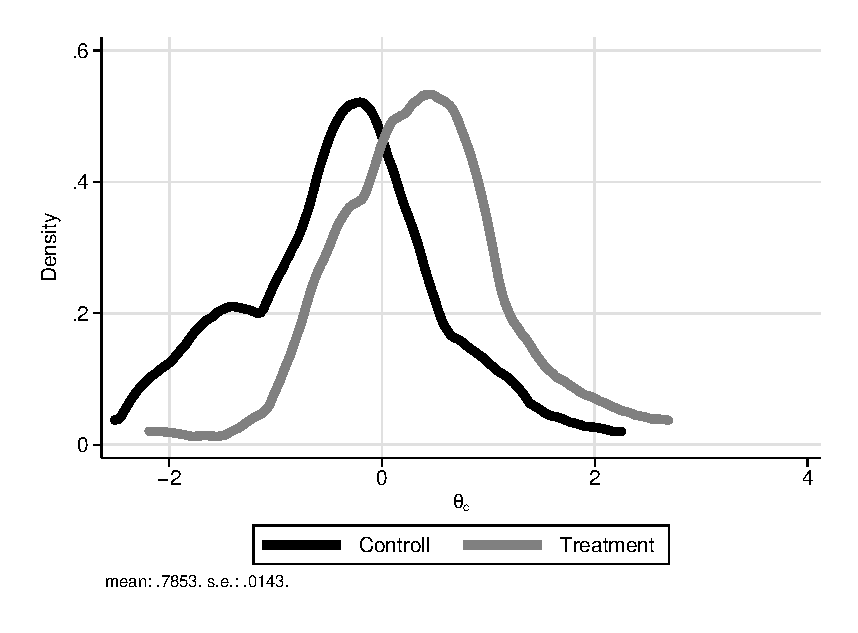
\includegraphics[width=\textwidth]{output/abccare_cfactor.eps}
\end{subfigure}%
\begin{subfigure}[h]{0.5\textwidth}
	\centering
	\caption{Non-cognitive} \label{fig:n}
		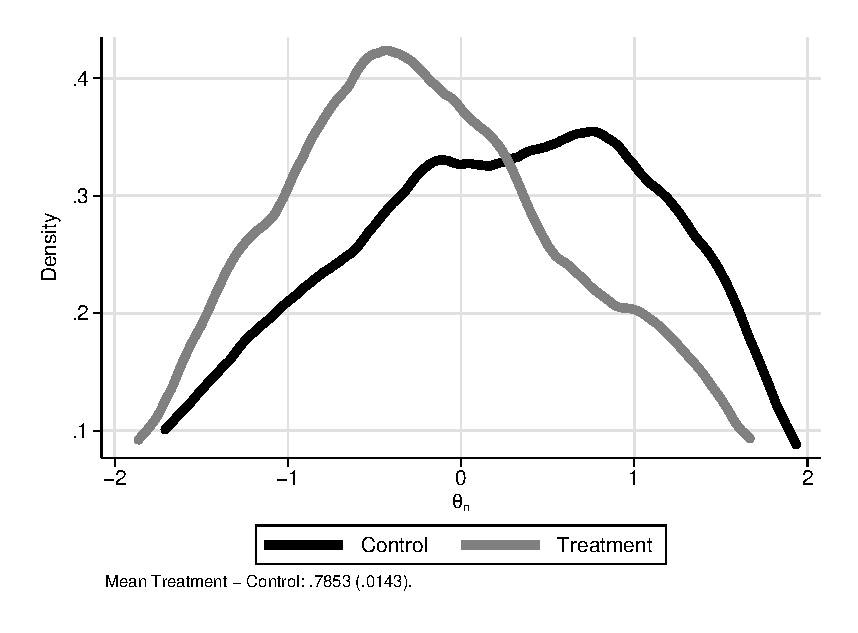
\includegraphics[width=\textwidth]{output/abccare_nfactor.eps}
\end{subfigure}
\footnotesize \justify
Note: Panels (a) displays a factor score estimated based on the measurement system in \eqref{eq:msystem} and measures of IQ at ages 2, 3, 4, 5, 7, and 8 (cognitive skill). Panel (b) displays an analogous exercise using measures measures of somatization, hostility, depression, and a global mental health index at age 21 (non-cognitive skill). Both measures of skills are standardized to a mean of $0$ and a standard deviation of $1$. ``Less'' in the factor measuring non-cognitive skills is ``positive'' given the measures we rely on to construct it. The mean difference between treatment and control is displayed below each panel, with standard error in parentheses. Standard errors are based on the bootstrap empirical distribution.
\end{figure}

\noindent Our tests of Assumption~\ref{ass:summary} display little sensitivity to controlling for $\bm{\theta}_{t}^d$. When constructing a system analogous to \eqref{eq:msystemmain} in the non-experimental sample to account for endogeneity, we also find little sensitivity to accounting for endogeneity when testing Assumption~\ref{ass:invariance} and when constructing predictions. These tests indicate that  $\left( \bm{X}_{t}, \bm{B} \right)$ are adequate measured inputs for the output $Y_{j,t}$ and that endogeneity is not a first order concern for our predictions (see Appendix~\ref{app:invariance} and Appendix~\ref{app:endogeneity}).\\

\noindent \textbf{[JLG: After this, I suggest to continue with what we currently have for Sections 6.3 to 6.6.]}

%References
\singlespace
\bibliographystyle{chicago}
\bibliography{heckman}

\end{document} 